\chapter{PackMime-HTTP: Web Traffic Generation}
\label{chap:packmime}

The PackMime Internet traffic model was developed by researchers in
the Internet Traffic Research group at Bell Labs, based on recent
Internet traffic traces.  PackMime includes a model of HTTP traffic,
called PackMime-HTTP. The traffic intensity generated by PackMime-HTTP
is controlled by the \emph{rate} parameter, which is the average number of
new HTTP connections started each second. The PackMime-HTTP implementation
in ns-2, developed at UNC-Chapel Hill, is capable of generating
HTTP/1.0 and HTTP/1.1 (persistent, non-pipelined) connections.

The goal of PackMime-HTTP is not to simulate the interaction between
a single web client and web server, but to simulate the TCP-level
traffic generated on a link shared by many web clients and servers.

A typical PackMime-HTTP instance consists of two ns nodes: a server
node and a client node.  It is important to note that these nodes \emph{do
not} correspond to a single web server or web client.  A single
PackMime-HTTP client node generates HTTP connections coming from a
``cloud'' of web clients.  Likewise, a single PackMime-HTTP server
node accepts and serves HTTP connections destined for a ``cloud'' of
web servers.  A single web client is represented by a single PackMime-HTTP
client application, and a single web server is represented by a single
PackMime-HTTP server application.  There are many client applications
assigned to a single client ns node, and many server applications
assigned to a single server ns node.

In order to simulate different RTTs, bottleneck links, and/or loss
rates for each connection, PackMime-HTTP is often used in conjunction
with DelayBox (see Chapter \ref{chap:delaybox}).  DelayBox is a module
developed at UNC-Chapel Hill for delaying and/or dropping packets in a
flow according to a given distribution.  See Section \ref{sec:pm-db} for
more information on using PackMime-HTTP and DelayBox together.

The PackMime HTTP traffic model is described in detail in the following paper:
J. Cao, W.S. Cleveland, Y. Gao, K. Jeffay, F.D. Smith, and M.C. Weigle
, ``Stochastic Models for Generating Synthetic HTTP Source Traffic'',
\emph{Proceedings of IEEE INFOCOM}, Hong Kong, March 2004.

\section{Implementation Details}
PackMimeHTTP is an ns object that drives the generation of HTTP
traffic. Each PackMimeHTTP object controls the operation of two types
of Applications, a PackMimeHTTP server Application and a PackMimeHTTP
client Application. Each of these Applications is connected to a TCP
Agent (Full-TCP).   {\bf Note:} PackMime-HTTP only supports Full-TCP
agents. 

\begin{figure}
\centering
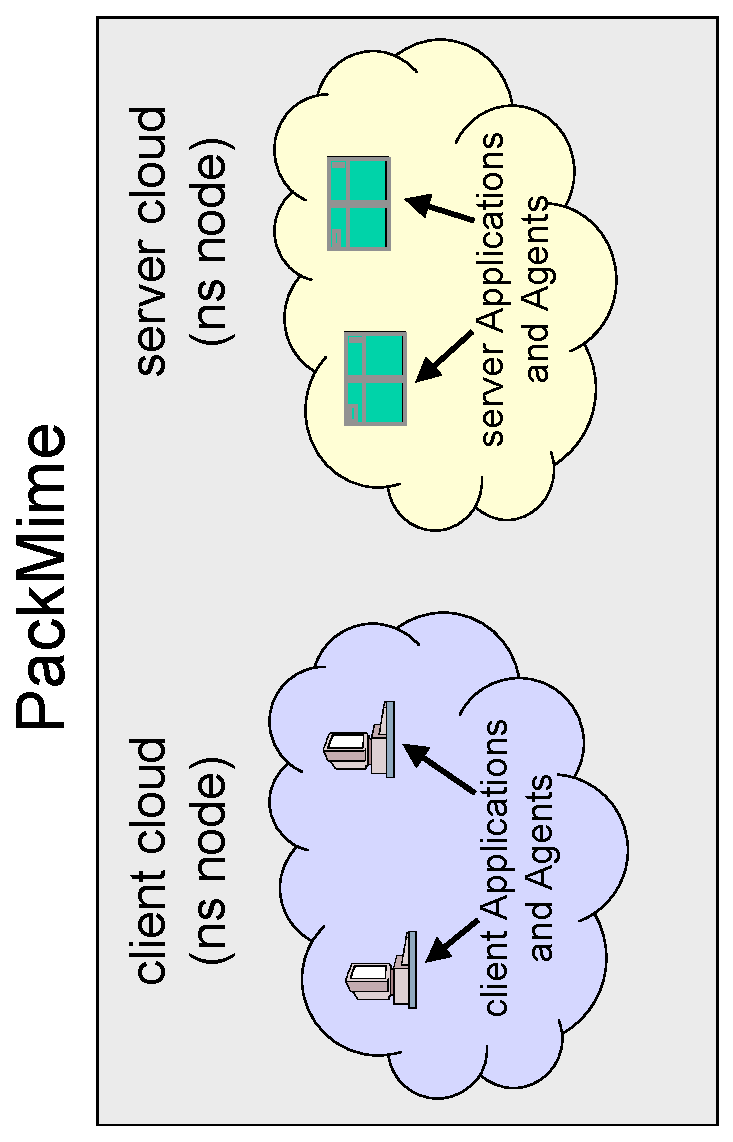
\includegraphics[scale=0.5, angle=270, clip]{packmime.eps}
\label{fig-pm}
\caption{PackMimeHTTP Architecture. Each PackMimeHTTP object controls
a server and a client cloud. Each cloud can represent multiple client
or server Applications. Each Application represents either a single
web server or a single web client.} 
\end{figure}  

Each web server or web client cloud is represented by a single ns node
that can produce and consume multiple HTTP connections at a time
(Figure \ref{fig-pm}). For each HTTP connection, PackMimeHTTP creates (or
allocates from the inactive pool, as described below) server and
client Applications and their associated TCP Agents. After setting up
and starting each connection, PackMimeHTTP sets a timer to expire when
the next new connection should begin. The time between new connections
is governed by the connection rate parameter supplied by the user. New
connections are started according to the connection arrival times
without regard to the completion of previous requests, but a new
request between the same client and server pair (as with HTTP 1.1)
begins only after the previous request-response pair has been
completed. 

PackMimeHTTP handles the re-use of Applications and Agents that have
completed their data transfer. There are 5 pools used to maintain
Applications and Agents -- one pool for inactive TCP Agents and one
pool each for active and inactive client and server Applications. The
pools for active Applications ensure that all active Applications are
destroyed when the simulation is finished. Active TCP Agents do not
need to be placed in a pool because each active Application contains a
pointer to its associated TCP Agent. New objects are only created when
there are no Agents or Applications available in the inactive pools. 

\subsection{PackMimeHTTP Client Application}

Each PackMimeHTTP client controls the HTTP request sizes that are
transferred. Each PackMimeHTTP client takes the following steps: 
\begin{itemize}
\item{if the connection is persistent and consists of more than one
  request, then the client samples all request sizes, response sizes,
  and inter-request times for the connection}
\item{if the connection only consists of one request, then the client
  samples the request size and the response size}
\item{send the first HTTP request to the server}
\item{listen for the HTTP response}
\item{when the entire HTTP response has been received, the client sets
a timer to expire when the next request should be made, if applicable}
\item{when the timer expires, the next HTTP request is sent, and the
above process is repeated until all requests have been completed}
\end{itemize}

\subsection{PackMimeHTTP Server Application}

Each web server controls the response sizes that are transferred. The
server is started by when a new TCP connection is started. Each
PackMimeHTTP client takes the following steps: 
\begin{itemize}
\item{listen for an HTTP request from the associated client}
\item{when the entire request arrives, the server samples the server
delay time from the server delay distribution} 
\item{set a timer to expire when the server delay has passed}
\item{when the timer expires, the server sends response (the size of
  which was sampled by the client and passed to the server)}
\item{this process is repeated until the requests are exhausted -- the
server is told how many requests will be sent in the connection} 
\item{send a FIN to close the connection}
\end{itemize}

\section{PackMimeHTTP Random Variables}

This implementation of PackMimeHTTP provides several ns RandomVariable
objects for specifying distributions of PackMimeHTTP connection
variables. The implementations were taken from source code provided by
Bell Labs and modified to fit into the ns RandomVariable
framework. This allows PackMimeHTTP connection variables to be
specified by any type of ns RandomVariable, which now include
PackMimeHTTP-specific random variables. If no RandomVariables are
specified in the TCL script, PackMimeHTTP will set these
automatically.  

The PackMimeHTTP-specific random variable syntax for TCL scripts is as
follows:  
\begin{itemize}
\item{{\tt \$ns [new RandomVariable/PackMimeHTTPFlowArrive <rate>]},
where {\tt rate} is the specified PackMimeHTTP connection rate (number  
of new connections per second)}
\item{{\tt \$ns [new RandomVariable/PackMimeHTTPReqSize <rate>]},
where {\tt rate} is the specified PackMimeHTTP connection rate} 
\item{{\tt \$ns [new RandomVariable/PackMimeHTTPRspSize <rate>]},
where {\tt rate} is the specified PackMimeHTTP connection rate}
\item{{\tt \$ns [new RandomVariable/PackMimeHTTPPersistRspSize]}}
\item{{\tt \$ns [new RandomVariable/PackMimeHTTPPersistent
    <probability>]},
where {\tt probability} is the probability that the connection is
    persistent} 
\item{{\tt \$ns [new RandomVariable/PackMimeHTTPNumPages <probability>
<shape> <scale>]}, where {\tt probability} is the probability that
  there is a single page in the connection and {\tt shape} and {\tt
    scale} are parameters to the Weibull distribution to determine the
number of pages in the connection.}
\item{{\tt \$ns [new RandomVariable/PackMimeHTTPSingleObjPages
      <probability>]}, where {\tt probability} is the probability that
      there is a single object on the current page.}
\item{{\tt \$ns [new RandomVariable/PackMimeHTTPObjsPerPage <shape>
      <scale>]}, where {\tt shape} and {\tt scale} are parameters to
      the Gamma distribution to determine the number of objects on a
      single page.}
\item{{\tt \$ns [new RandomVariable/PackMimeHTTPTimeBtwnObjs]}}
\item{{\tt \$ns [new RandomVariable/PackMimeHTTPTimeBtwnPages]}}
\item{{\tt \$ns [new RandomVariable/PackMimeHTTPServerDelay <shape>
      <scale>]}, where {\tt shape} and {\tt scale} are paramters to
      the Weibull distribution to determine server delay.}
\item{{\tt \$ns [RandomVariable/PackMimeHTTPXmit <rate> <type>]}, where
{\tt type} is 0 for client-side delays and 1 for
server-side delays.  \textbf{Note:} This random variable
is only used in conjunction with DelayBox.  It returns 1/2 of the
actual delay because it is meant to be used with 2 DelayBox nodes,
each of which should delay the packets for 1/2 of the actual delay.} 
\end{itemize}

\section{Use of DelayBox with PackMime-HTTP}
\label{sec:pm-db}

\begin{figure}
\centering
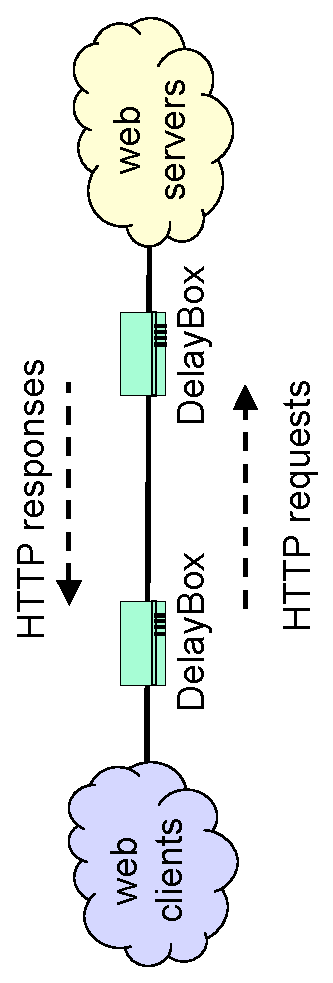
\includegraphics[scale=0.75,angle=270, clip]{packmime-delaybox.eps}
\label{fig-pmdb}
\caption{Example Topology Using PackMimeHTTP and DelayBox. The cloud
  of web clients is a single ns node, and the cloud of web servers is
  a single ns node. Each of the DelayBox nodes is a single ns node.} 
\end{figure}  

PackMimeHTTP uses ns to model the TCP-level interaction between web
clients and servers on the simulated link. To simulate network-level
effects of HTTP transfer through the clouds, use DelayBox (see
\ref{chap:delaybox}). DelayBox is an ns analog to dummynet, often used
in network testbeds to delay and drop packets. The delay times model
the propagation and queuing delay incurred from the source to the edge
of the cloud (or edge of the cloud to destination). Since all HTTP
connections in PackMimeHTTP take place between only two ns nodes,
there must be an ns object to delay packets in each flow, rather
than just having a static delay on the link between the two
nodes. DelayBox also models bottleneck links and packet loss on an
individual connection basis. Two DelayBox nodes are used as shown in
Figure \ref{fig-pmdb}. One node is placed in front of the web client
cloud ns node to handle client-side delays, loss, and bottleneck
links. The other DelayBox node is placed in front of the web server
cloud ns node to handle the server-side delays, loss, and bottleneck
links.

\section{Example}
More examples (including those that demonstrate the use of DelayBox
with PackMime) are available in the {\tt tcl/ex/packmime/} directory of the
ns source code.  The validation script {\tt test-suite-packmime.tcl}
is in {\tt tcl/test/} and can be run with the command {\tt
test-all-packmime} from that directory.

\textbf{Note:}  The only PackMime-HTTP parameters that \emph{must} be set are
       {\tt rate}, {\tt client}, {\tt server}, {\tt flow\_arrive}, {\tt
       req\_size}, and {\tt rsp\_size}.  The example below shows the
       minimal parameters that need to be set, but other parameters
       can be set to change the default behavior (see ``Commands at a
       Glance'').  

\begin{verbatim}
# test-packmime.tcl

# useful constants
set CLIENT 0
set SERVER 1

remove-all-packet-headers;             # removes all packet headers
add-packet-header IP TCP;              # adds TCP/IP headers
set ns [new Simulator];                # instantiate the Simulator
$ns use-scheduler Heap;                # use the Heap scheduler

# SETUP TOPOLOGY
# create nodes
set n(0) [$ns node]
set n(1) [$ns node]
# create link
$ns duplex-link $n(0) $n(1) 10Mb 0ms DropTail

# SETUP PACKMIME
set rate 15
set pm [new PackMimeHTTP]
$pm set-client $n(0);                  # name $n(0) as client
$pm set-server $n(1);                  # name $n(1) as server
$pm set-rate $rate;                    # new connections per second
$pm set-http-1.1;                      # use HTTP/1.1

# SETUP PACKMIME RANDOM VARIABLES
global defaultRNG

# create RNGs (appropriate RNG seeds are assigned automatically)
set flowRNG [new RNG]
set reqsizeRNG [new RNG]
set rspsizeRNG [new RNG]

# create RandomVariables
set flow_arrive [new RandomVariable/PackMimeHTTPFlowArrive $rate]
set req_size [new RandomVariable/PackMimeHTTPFileSize $rate $CLIENT]
set rsp_size [new RandomVariable/PackMimeHTTPFileSize $rate $SERVER]

# assign RNGs to RandomVariables
$flow_arrive use-rng $flowRNG
$req_size use-rng $reqsizeRNG
$rsp_size use-rng $rspsizeRNG

# set PackMime variables
$pm set-flow_arrive $flow_arrive
$pm set-req_size $req_size
$pm set-rsp_size $rsp_size

# record HTTP statistics
$pm set-outfile "data-test-packmime.dat"

$ns at 0.0 "$pm start"
$ns at 30.0 "$pm stop"

$ns run
\end{verbatim}

\section{Commands at a Glance}
The following commands on the PackMimeHTTP class can be accessed from OTcl:

{\tt [new PackMimeHTTP]}\\
Creates a new PackMimeHTTP object.

{\tt \$packmime start}\\
Start generating connections

{\tt \$packmime stop}\\
Stop generating new connections

{\tt \$packmime set-client <node>}\\
Associates the node with the PackMimeHTTP client cloud 

{\tt \$packmime set-server <node>}\\
Associates the node with the PackMimeHTTP server cloud 

{\tt \$packmime set-rate <float>}\\
Set the average number of new connections started per second 

{\tt \$packmime set-req\_size <RandomVariable>}\\
Set the HTTP request size distribution 

{\tt \$packmime set-rsp\_size <RandomVariable>}\\
Set the HTTP response size distribution 

{\tt \$packmime set-flow\_arrive <RandomVariable>}\\
Set the time between two consecutive connections starting

{\tt \$packmime set-server\_delay <RandomVariable>}\\
Set the web server delay for fetching pages 

{\tt \$packmime set-run <int>}\\
Set the run number so that the RNGs used for the random variables will
use the same substream (see Chapter \ref{chap:math} on RNG for more details).

{\tt \$packmime get-pairs}\\
Return the number of completed HTTP request-response pairs.  See 
{\tt tcl/ex/packmime/pm-end-pairs.tcl} for an example of using
{\tt get-pairs} to end the simulation after a certain number of
pairs have completed.

{\tt \$packmime set-TCP <protocol>}\\
Sets the TCP type (Reno, Newreno, or Sack) for all connections in the
client and server clouds - Reno is the default

{\bf HTTP/1.1-Specific Commands}

{\tt \$packmime set-http-1.1}\\
Use HTTP/1.1 distributions for persistent connections instead of HTTP/1.0.

{\tt \$packmime no-pm-persistent-reqsz}\\
By default, PackMime-HTTP sets all request sizes in a persistent
connection to be the same. This option turns that behavior off and
samples a new request size from the request size distribution for each
request in a persistent connection.

{\tt \$packmime no-pm-persistent-rspsz}\\
By default, PackMime-HTTP uses an algorithm (see {\tt
  PackMimeHTTPPersistRspSizeRandomVariable::value()} in {\tt
  packmime\_ranvar.h} for details) for setting the response sizes in a
persistent connection.  This option turns that behavior off and
samples a new response size from the response size distribution for
each response in a persistent connection.

{\tt \$packmime set-prob\_persistent <RandomVariable>}\\
Set the probability that the connection is persistent

{\tt \$packmime set-num\_pages <RandomVariable>}\\
Set the number of pages per connection

{\tt \$packmime set-prob\_single\_obj <RandomVariable>}\\
Set the probability that the page contains a single object

{\tt \$packmime set-objs\_per\_page <RandomVariable>}\\
Set the number of objects per page

{\tt \$packmime set-time\_btwn\_pages <RandomVariable>}\\
Set the time between page requests (\emph{i.e.}, think time)

{\tt \$packmime set-time\_btwn\_objs <RandomVariable>}\\
Set the time between object requests

{\bf Output-Specific Commands}

{\tt \$packmime active-connections}\\
Output the current number of active HTTP connections to standard error 

{\tt \$packmime total-connections}\\
Output the total number of completed HTTP connections to standard error

{\tt \$packmime set-warmup <int>}\\
Sets what time output should start.  Only used with {\tt set outfile}.

{\tt \$packmime set-outfile <filename>}\\
Output the following fields (one line per HTTP request-reponse pair)
to {\tt filename}:
\begin{itemize}
\item{time HTTP response completed}
\item{HTTP request size (bytes)}
\item{HTTP response size (bytes)}
\item{HTTP response time (ms) -- time between client sending HTTP
request and client receiving complete HTTP response} 
\item{source node and port identifier}
\item{number of active connections at the time this HTTP
request-response pair completed}
\end{itemize}

{\tt \$packmime set-filesz-outfile <filename>}\\
Right after sending a response, output the following fields (one line
per HTTP request-reponse pair) to {\tt filename}: 
\begin{itemize}
\item{time HTTP response sent}
\item{HTTP request size (bytes)}
\item{HTTP response size (bytes)}
\item{server node and port address}
\end{itemize}

{\tt \$packmime set-samples-outfile <filename>}\\
Right before sending a request, output the following fields (one line
per HTTP request-reponse pair) to {\tt filename}: 
\begin{itemize}
\item{time HTTP request sent}
\item{HTTP request size (bytes)}
\item{HTTP response size (bytes)}
\item{server node and port address}
\end{itemize}

{\tt \$packmime set-debug <int>}\\
Set the debugging level:
\begin{itemize}
\item{1: Output the total number of connections created at the end of
the simulation}
\item{2: Level 1 + \\
output creation/management of TCP agents and applications\\
output on start of new connection\\
number of bytes sent by the client and expected response size\\
number of bytes sent by server}
\item{3: Level 2 + \\
output when TCP agents and applications are moved to the pool}
\item{4: Level 3 + \\
output number of bytes received each time client or server receive a packet}
\end{itemize}



